\chapter{Das Registrierungsformular}

Der wohl komplizierteste Teil dieser Diplomarbeit ist der Aufbau und die korrekte Validierung des Registrierungsformulars. Das Ziel ist den Benutzern eine möglichst einfache und schnelle Registrierung, unter Berücksichtigung des derzeitigen Standorts und der dazugehörigen Benutzergruppe, anzubieten. Dafür wurde ein Algorithmus entwickelt, welcher bei der \texttt{ngAfterViewInit} Lifecycle-Hook-Methode im \texttt{UserprofileComponent} seinen Start nimmt.

\section{Der Algorithmus hinter dem dynamischen Aufbau}

\begin{figure}[H]
	\centerline{
		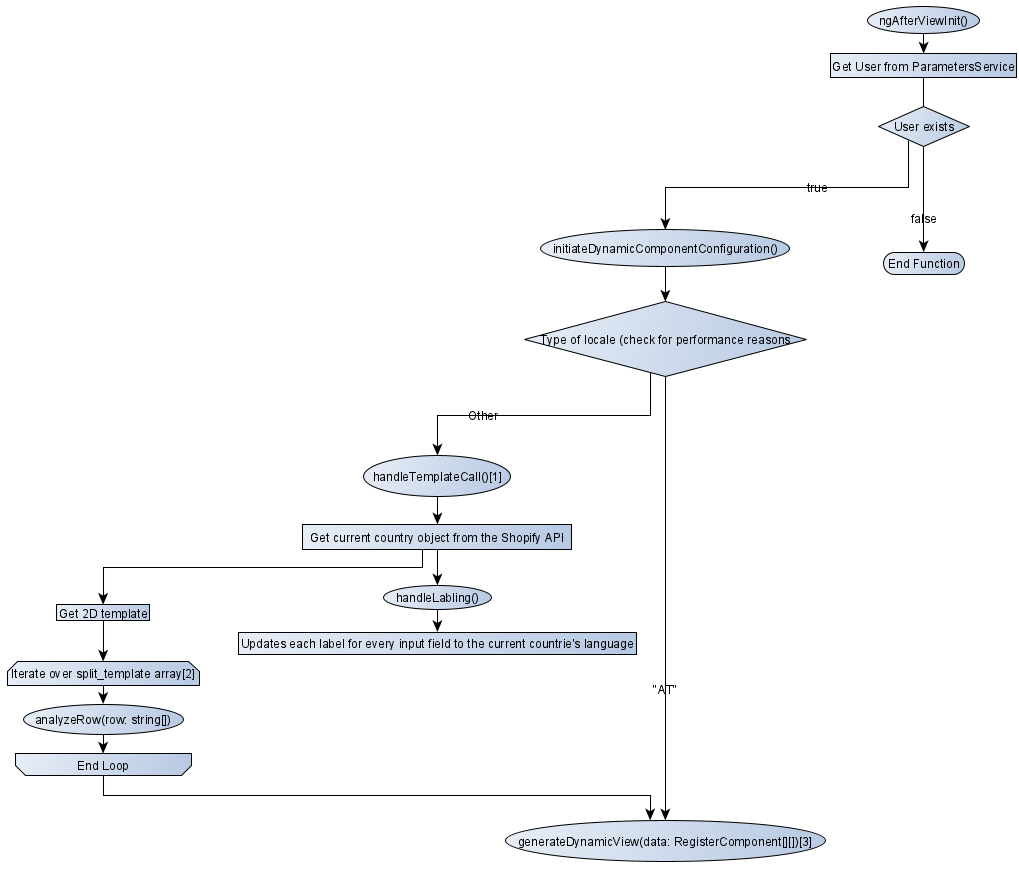
\includegraphics[width=1\textwidth, frame]{./grafiken/RF_Flussdiagramm.png}
	}
	\vskip0pt
	\caption{Flussdiagramm des Algorithmus}
\end{figure}

Wenn das User-Objekt, welches von der Backend API abgefragt und erfolgreich als globale Objekt variable gespeichert wurde, wird die \texttt{initiateDynamicComponentConfigu\\ration()}-Methode aufgerufen. Aus Performance-Gründen basiert die nächste Überprüfung auf den Wert der aktuellen Lokale. Gleicht dieser den Wert "AT", so wird ein vorgefertigtes Template für ein österreichisches RF, dargestellt im Listing~\ref{lst:template_form_aut}, für die Weiterverwendung benützt. Da davon ausgegangen wird, dass sich vor allem in der Anfangsphase nach der Veröffentlichung hauptsächlich österreichische Kunden ein Konto erstellen, spart dieser Weg enorm viel Zeit, da sofort mit der Erstellung des RF begonnen werden kann.

\begin{lstlisting}[caption={Vordefiniertes Template für das RF},captionpos=b, language=JavaScript,label={lst:template_form_aut}]
export const AUSTRIAN_PRIVATE_PERSON_FORM_Template = [
	[{ type: GenderComponent }],
	[
		{ type: FirstnameComponent, options: { label: "Vorname" } },
		{ type: LastnameComponent, options: { label: "Nachname" } },
	],
	[{ type: StreetComponent, options: { label: "Straße und Hausnummer" } }],
	[
		{ type: CityComponent, options: { label: "Stadt" } },
		{ type: PostalcodeComponent, options: { label: "Postleitzahl" } },
	],
	[
	{
		type: PhoneComponent,
		options: { label: "Telefonnummer", phonePrefix: 43 },
	},
	{ type: DateofbirthComponent },
	],
];
\end{lstlisting}

Anderenfalls wird als nächster Schritt die \texttt{handleTemplateCall()}-Methode aufgerufen, welche, basierend auf den Wert der aktuellen Lokale, auf die Shopify API zugreift, um ein \texttt{Country}-Objekt abzurufen. Wurde diese Operation beendet folgt ein Update auf die Labels für den Wrapper der Objekte für das RF. Nach dem das Template geladen wurde wird über jedes einzelne Element iteriert um daraus eine oder mehrere Zeilen zu generieren um diese in ein 2D Array zu speichern. 

\begin{lstlisting}[caption={Erstellung des 2D Arrays für den Aufbau des RF},captionpos=b, language=JavaScript,label={lst:analyzeRow}]
private analyzeRow(row: string[]): RegisterComponent[][] {
	let addGenderC = false;
	let result: RegisterComponent[][] = [];
	let componentRow: RegisterComponent[] = [];
	
	for (let i = 0; i < row.length; i++) {
		let rowEl = row[i];
		
		if (!addGenderC) {
			if (rowEl.includes("firstName") || rowEl.includes("lastName")) {
				let genderComponent: RegisterComponent[] = [
				{ type: GenderComponent },
				];
				result.push(genderComponent);
				addGenderC = true;
			}
		}
		
		if (rowEl.includes("company") && this.user.isPrivatePerson) {
			break;
		}
		
		for (const x of this.valueMap.keys()) {
			if (rowEl.includes(x)) {
				let compEl: RegisterComponent = {
					type: this.valueMap.get(x),
				};
				
				if (
				compEl.type.prototype ===
				ZoneComponent.prototype
				) {
					compEl.options.zones = this.countryFromService.zones.map(
					(x) => x.name
					);
					this.user.zone = compEl.options.zones[0];
				}
				
				if (
				compEl.type.prototype ===
				PhoneComponent.prototype
				) {
					compEl.options.phonePrefix = this.countryFromService.phoneNumberPrefix;
				}
				
				if (this.labels.get(x)) {
					compEl.options.label = this.labels.get(x);
				}
				
				componentRow.push(compEl);
				if (rowEl.includes("phone")) {
					let dateofbirthComponent: RegisterComponent = {
						type: DateofbirthComponent,
					};
					componentRow.push(dateofbirthComponent);
				}
				break;
			}
		}
	}
	result.push(componentRow);
	return result;
}
\end{lstlisting}

Die im Listing~\ref{lst:analyzeRow}


\section{Die Validierungsmethodik}

\section{Die Komfortfunktionen}

\begin{figure}[H]
	\centerline{
		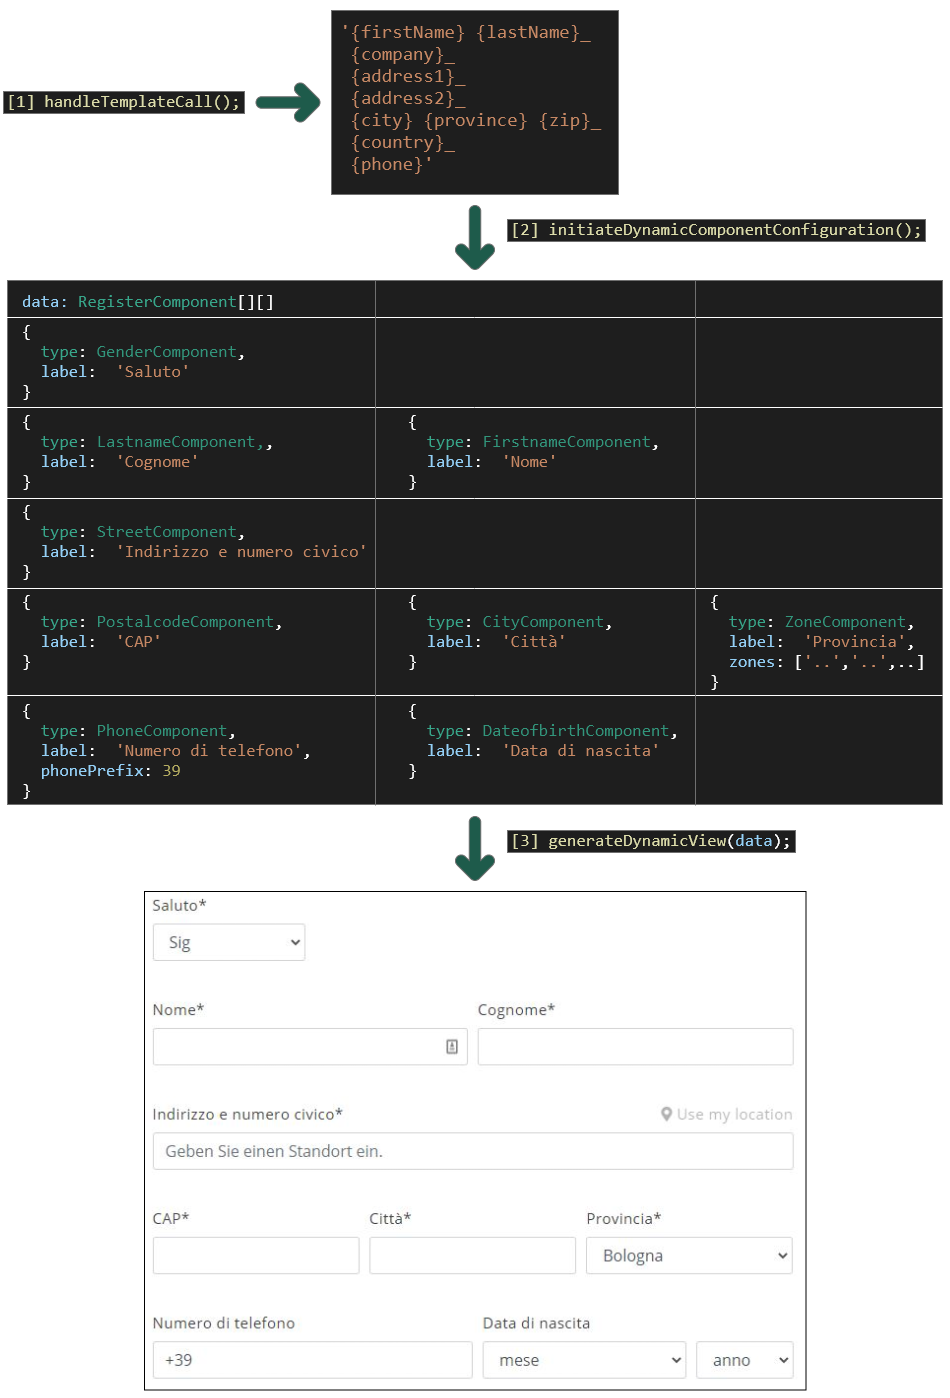
\includegraphics[width=1\textwidth, frame]{./grafiken/RF_Datenvisualisierung.png}
	}
	\vskip0pt
	\caption{Visualisierter Datenfluss vom Template bis zum fertigen RF}
\end{figure}

